%-------------------------------------------------------------------------------
% ICML Workshop Paper: Meta-Learning for Boolean Concept Induction
%-------------------------------------------------------------------------------
\documentclass{article}
% Common packages
\usepackage[utf8]{inputenc}
\usepackage{amsmath, amssymb, amsfonts}
\usepackage{graphicx}
\usepackage[numbers,sort&compress]{natbib} % Using numbers and compress for space, common in ICML.
\usepackage{hyperref} % Should generally be loaded later
\usepackage{booktabs} % For better tables
\usepackage[margin=1in]{geometry} % Standard margins

% Specific packages for figures and layout
\usepackage{tikz}
\usetikzlibrary{shapes.geometric, arrows.meta, positioning, fit}
\usepackage{float} % For [H] figure placement specifier
% \usepackage{wrapfig} % For wrapfigure environment - REMOVED as AUC plot is removed

\usepackage[font=small,skip=5pt]{caption} % Smaller captions, less skip

\title{Adapting to High Dimensional Concepts with Metalearning}

\author{%
  Author Names Withheld \\\\\\\\ % Use \\\\ for a new line
  % Affiliation Withheld \\\\ % Add affiliation if desired
  Under Review for the Workshop on High-dimensional Learning Dynamics, ICML 2025
}
\date{} % No date

\begin{document}
\maketitle

\begin{abstract}
Rapidly learning abstract rules from limited examples is a hallmark of human intelligence. This work investigates whether gradient-based meta-learning can equip neural networks with inductive biases for efficient few-shot acquisition of compositional Boolean concepts. We compare meta-learning strategies against a supervised learning baseline on Boolean tasks generated by a probabilistic context-free grammar, varying concept complexity and input dimensionality. Using a consistent multilayer perceptron (MLP) architecture, we evaluate performance based on final validation accuracy and learning efficiency. Our findings indicate that meta-learning, particularly when allowed more adaptation steps, offers significant advantages in data efficiency and final performance on lower-dimensional tasks. However, all methods face challenges as input dimensionality and concept complexity increase, highlighting the intricate interplay between learning strategies, task structure, and data representation in high-dimensional settings.
\end{abstract}

%===============================================================================
\section{Introduction}
Humans excel at few-shot concept learning, inferring abstract logical rules from minimal evidence \citep{Lake2015bpl}. Meta-learning algorithms, such as Model-Agnostic Meta-Learning (MAML; \citealp{Finn2017maml}) and its derivatives, aim to instill similar capabilities in neural networks by learning an initialization optimized for rapid adaptation. While effective in perceptual domains, their efficacy on structured, rule-based problems, especially those involving symbolic composition and high-dimensional inputs, remains an active research area. This study addresses this gap by asking: \emph{How do meta-learning strategies and standard supervised learning compare in acquiring PCFG-generated Boolean concepts as a function of concept complexity?} We analyze learning dynamics through classification performance and data efficiency, contributing to the understanding of meta-learning dynamics in high-dimensional concept spaces.

%===============================================================================
\section{Related Work}\label{sec:related}
\textbf{Gradient-based meta-learning.} Meta-SGD \citep{Li2017metasgd} extends MAML by also learning per-parameter learning rates. First-order approximations (e.g., FOMAML, Reptile \citep{Nichol2018firstorder}) reduce computational costs by omitting Hessian calculations. The number of inner-loop adaptation steps ($K_{adapt}$) is a crucial hyperparameter, with more steps potentially allowing for finer-grained task-specific adjustments at the cost of increased computation during meta-training and adaptation \citep{Finn2017maml}. Theoretical work suggests that second-order methods, by capturing curvature, can act as a contrastive regularizer \citep{Kao2022contrastive}. We empirically test these trade-offs for symbolic concept induction, varying both the order and the number of adaptation steps as we sample concepts.

\textbf{Compositional concept learning.} Inducing symbolic rules has been approached via methods requiring explicit grammars and search \citep{Goodman2008lot, Lake2015bpl}. Recent efforts aim to bridge symbolic reasoning with neural approaches. Our work utilizes a purely Boolean setting, removing perceptual complexity to isolate the learning of compositional logical structure, with a specific focus on the impact of input dimensionality and adaptation strategy.

%===============================================================================
\section{Experimental Setup}\label{sec:methods}
Our experimental setup starts with a concept-generating Probabilistic Context-Free Grammar (PCFG) from Goodman et al. 2008 \citep{Goodman2008lot}. We modify the PCFG to explicitly control concept complexity via recursion depth ($D \in \{3, 5, 7\}$) and feature dimensionality (the number of literals $F \in \{8, 16, 32\}$). The grammar production rule is defined recursively : $C \to L \,|\, \neg C \,|\, (C \wedge C) \,|\, (C \vee C)$; where $L \to x_i$, over $F$ binary features $\mathcal{X}=\{x_1,\dots,x_F\}$. For instance, with $F=4$ features (e.g., $x_1, x_2, x_3, x_4$) and a target depth $D=3$, a sampled concept $C$ might be $\neg ((x_1 \wedge x_2) \vee (\neg x_3))$. Such concepts define a binary function $C(\mathbf{x})$ which evaluates to true or false for any given input vector $\mathbf{x} \in \{0,1\}^F$. For each task $C$, a $K_{shot}$ support set $S_C$ ($K_{shot}=5$ positive and $K_{shot}=5$ negative examples $(\mathbf{x}, C(\mathbf{x}))$) and a query set $Q_C$ are generated from uniformly sampled $\mathbf{x} \in \{0,1\}^F$.


\begin{figure}[ht]
\centering
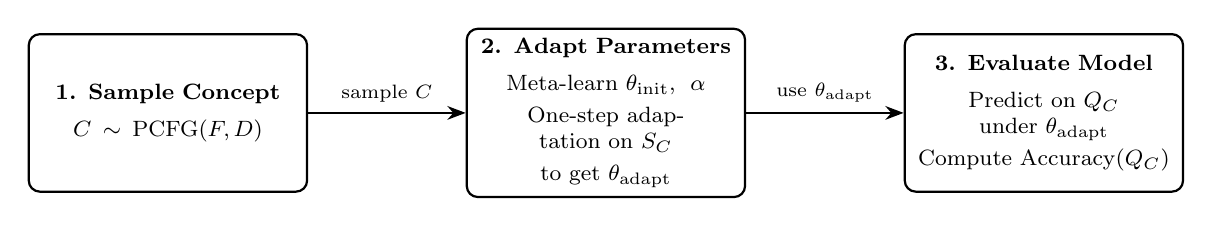
\begin{tikzpicture}[
  node distance=15mm and 20mm,
  stage/.style={
    draw, thick, rounded corners,
    minimum width=3.5cm, minimum height=2cm,
    align=center, font=\footnotesize, text width=3.3cm
  },
  arr/.style={-{Stealth[scale=1]}, thick}
]

% 1. Sampling node
\node[stage] (sample) {
  \textbf{1. Sample Concept} \\[4pt]
  $C \sim \mathrm{PCFG}(F,D)$
};

% 2. Adaptation node
\node[stage, right=of sample] (adapt) {
  \textbf{2. Adapt Parameters} \\[4pt]
  Meta-learn $\theta_{\mathrm{init}},\;\alpha$ \\[2pt]
  One-step adaptation on $S_C$ \\[2pt]
  to get $\theta_{\mathrm{adapt}}$
};

% 3. Evaluation node
\node[stage, right=of adapt] (eval) {
  \textbf{3. Evaluate Model} \\[4pt]
  Predict on $Q_C$ under $\theta_{\mathrm{adapt}}$ \\[2pt]
  Compute $\mathrm{Accuracy}(Q_C)$
};

% Arrows
\draw[arr] (sample) -- node[above, font=\scriptsize]{sample $C$} (adapt);
\draw[arr] (adapt) -- node[above, font=\scriptsize]{use $\theta_{\mathrm{adapt}}$} (eval);

\end{tikzpicture}
\caption{The three-stage meta-learning pipeline. 1. A Boolean concept $C$ is sampled from a PCFG (features $F$, depth $D$). 2. Meta-learned initial parameters $\theta_{init}$ and per-parameter learning rates $\alpha$ are adapted on a support set $S_C$ for $K_{adapt}$ gradient steps to yield $\theta_{adapt}$. 3. The adapted model $\theta_{adapt}$ is evaluated on a query set $Q_C$.}\label{fig:meta_episode}
\end{figure}

All methods use a 5-layer MLP (128 hidden units/layer, ReLU, sigmoid output). We compare models trained with four learning algorithms:
\begin{itemize}
    \item \textbf{1st-Order Meta-SGD ($K_{adapt}=1$)}: Meta-gradients ignore Hessians; one adaptation step.
    \item \textbf{2nd-Order Meta-SGD ($K_{adapt}=1$)}: Uses full Hessian-vector products; one adaptation step.
    \item \textbf{1st-Order Meta-SGD ($K_{adapt}=10$)}: Meta-gradients ignore Hessians; ten adaptation steps.
    \item \textbf{Supervised SGD}: MLP trained from scratch per task using Adam \citep{Kingma2014adam} (LR 0.001) on $S_C$.
\end{itemize}

During adaptation for Meta-SGD variants, the parameters $\theta$ are updated for $K_{adapt}$ steps. Starting with $\theta^{(0)} = \theta_{init}$ (the meta-learned initialization), for each step $k \in \{0, \dots, K_{adapt}-1\}$, the update is:
\[
\theta^{(k+1)} = \theta^{(k)} - \alpha \odot \nabla_{\theta^{(k)}} \mathcal{L}_{S_C}(\theta^{(k)}) \label{eq:adapt_step}
\]
where $\alpha$ are the meta-learned per-parameter learning rates and $\mathcal{L}_{S_C}$ is the loss (binary cross-entropy) on the support set $S_C$. The final adapted parameters are $\theta_{adapt} = \theta^{(K_{adapt})}$. Increasing $K_{adapt}$ allows the model to perform a more extensive search in the task-specific loss landscape, potentially finding a solution that better minimizes the empirical risk on $S_C$. For Boolean concepts, this translates to a more refined adjustment of the MLP's decision boundaries to correctly classify the examples in the support set.

Meta-SGD models were meta-trained for 10,000 episodes. All evaluations were averaged over 5 random seeds on 1,000 unseen tasks. For trajectory comparisons, SGD is trained for steps equivalent to processing a fixed total number of samples.

Performance is assessed using: \textbf{1. Final Mean Accuracy} (see Appendix~\ref{app:final_acc_bar} for summary bar chart, Figure~\ref{fig:final_accuracy_bar_appendix}); and \textbf{2. Data Efficiency}: The number of training samples (episodes for MetaSGD, scaled appropriately for SGD) required to reach a threshold accuracy of 60\% (Figure~\ref{fig:data_efficiency_samples_to_threshold}).

%===============================================================================
\section{Results}\label{sec:results}
We present findings across varying feature dimensionalities ($F$) and concept depths ($D$), averaged over 5 seeds.

Figure~\ref{fig:accuracy_trajectories} shows the learning trajectories. Meta-SGD methods demonstrate a clear advantage over SGD from scratch, learning faster and converging to higher accuracies, particularly for $F=8$ and $F=16$. The \texttt{MetaSGD\_1stOrd\_K10} variant is particularly noteworthy, often matching or exceeding the performance of \texttt{MetaSGD\_2ndOrd\_K1}, especially in terms of learning speed. This suggests that increasing the number of first-order adaptation steps can be a highly effective strategy. Final validation accuracies are summarized in Appendix~\ref{app:final_acc_bar} (Figure~\ref{fig:final_accuracy_bar_appendix}), confirming these trends.

\begin{figure}[htbp!]
    \centering
    \includegraphics[width=0.75\linewidth]{Figures/plot_summary_combined_val_accuracy_faceted.png} % Ensure this path is correct
    \caption{Mean Validation Accuracy Trajectories. Comparison of Meta-SGD variants (K1 and K10 for 1st-Order, K1 for 2nd-Order) and SGD across features (rows) and concept depths (columns) over normalized training episodes. \texttt{MetaSGD\_1stOrd\_K10} often learns fastest and achieves competitive or superior accuracy to \texttt{MetaSGD\_2ndOrd\_K1}.}
    \label{fig:accuracy_trajectories}
\end{figure}

The benefit of meta-learning and increased adaptation steps is further highlighted by the data efficiency plot (Figure~\ref{fig:data_efficiency_samples_to_threshold}). MetaSGD methods require substantially fewer samples to reach the 60\% accuracy threshold compared to SGD. \texttt{MetaSGD\_1stOrd\_K10} is often the most data-efficient, demonstrating that more adaptation steps enable the model to more rapidly specialize to the task at hand using the limited support set. For instance, at $F=8, D=3$, \texttt{MetaSGD\_1stOrd\_K10} reaches the threshold with orders of magnitude fewer samples than SGD.

As input dimensionality increases to $F=32$, all methods exhibit a significant drop in performance across all metrics. While Meta-SGD variants still maintain an edge over SGD, the absolute accuracies are much lower, and the data efficiency gains are less pronounced relative to the sheer number of samples still required. Notably, even in this high-dimensional regime ($F=32$), the \texttt{MetaSGD\_1stOrd\_K10} strategy tends to yield the largest relative performance improvements over its 1-step counterparts (both 1st and 2nd order Meta-SGD), suggesting that the benefit of more extensive adaptation becomes even more crucial when the search space is larger, underscoring the challenges of high-dimensional, few-shot learning.

\begin{figure}[htbp!]
    \centering
    \includegraphics[width=0.35\linewidth]{Figures/plot_samples_to_threshold_60pct_concept.png} % Ensure this path is correct.
    \caption{Data Efficiency: Training Samples to Reach 60\% Validation Accuracy (Log Scale). Lower values indicate higher efficiency. MetaSGD methods, especially \texttt{MetaSGD\_1stOrd\_K10}, are significantly more data-efficient than SGD.}
    \label{fig:data_efficiency_samples_to_threshold}
\end{figure}

%===============================================================================
\section{Discussion}\label{sec:discussion}
Our comparative analysis reveals several nuances in applying meta-learning algorithms to few-shot Boolean concept induction. Meta-learning, via Meta-SGD, generally offers substantial advantages over standard supervised training (SGD from scratch) in both final validation accuracy (Figure~\ref{fig:accuracy_trajectories} and Appendix~\ref{app:final_acc_bar}) and data efficiency (Figure~\ref{fig:data_efficiency_samples_to_threshold}). This benefit is particularly evident for the model trained with a larger number of adaptation steps, which often achieves performance comparable or superior to the 2nd-order variant but with only first-order gradient computations during adaptation. This suggests that providing the meta-learned initialization ($\theta_{init}, \alpha$) with more opportunity to fine-tune to the specific task $S_C$ (via $K_{adapt}=10$ steps) is highly effective for Boolean concept learning.

Comparing Meta-SGD variants, 2nd-order Meta-SGD often yields a modest improvement over first order (both with one adaptation step). However, first order with 10 adaptation steps outperforms across the board, especially with higher dimensional concepts. This indicates that for these tasks, the benefit of additional adaptation steps can outweigh the benefit of second-order information in a single adaptation step. The increased number of gradient updates (Equation~\ref{eq:adapt_step}) allows the model to more thoroughly explore the local loss landscape defined by $S_C$, leading to better task-specific parameters $\theta_{adapt}$.

The most striking finding remains the dramatic performance degradation across all methods when input dimensionality ($F$) increases to 32. The challenge stems from extreme data sparsity: $2K_{shot}=10$ examples from $2^{32}$ possible feature combinations. This highlights the "curse of dimensionality" as a critical bottleneck. Revisiting the results from Figure 2 in this context, the tendencies of meta-SGD suggest that a greater number of adaptation steps may be particularly vital when the feature space is exceptionally complex and high-dimensional. 

Pronounced difficulties at $F=32$ underscore the need for more robust methodologies. Future work could explore varying model capacity with increased feature complexity as well as other sources of inductive bias other than the weigth space, which we show to be a powerful inductive bias on even small, capacity constrained MLP's. We highlight this technique of weight initialization via metalearning as a promising path towards neural networks that can better reason compositionally and conceptually. 

%===============================================================================
\section{Conclusion}
This study presented a comparative empirical analysis of different meta-learning strategies and standard supervised SGD on a suite of few-shot Boolean concept induction tasks. Our findings affirm that meta-learning approaches can significantly enhance both final performance and data efficiency. Notably, increasing the number of adaptation steps and the order of the gradients used in metalearning proved to be a highly effective mechanism for improving few-shot learning in this domain. 

A principal contribution is the observation that, as featural dimensionality and sparsity increase linearly, and concept complexity increases exponentially, we need new sources of inductive bias to guide learning. Addressing these limitations by developing methods more robust to data sparsity in high dimensions is pivotal for advancing machine learning towards more human-like concept acquisition, and an area we are excited about developing. 

%===============================================================================
% References
%===============================================================================
\newpage % Ensure references start on a new page, helps with page count.
{\small
\bibliographystyle{plainnat}
\bibliography{ref}
}

%===============================================================================
% Appendix
%===============================================================================
\newpage
\appendix
\section{Appendix}

\subsection{Final Mean Validation Accuracy (Bar Chart)}\label{app:final_acc_bar}
This plot (Figure~\ref{fig:final_accuracy_bar_appendix}) complements the trajectory data in Figure~\ref{fig:accuracy_trajectories} by providing a direct comparison of final performance levels across the different learning methods and task configurations.
\begin{figure}[H]
    \centering
    \includegraphics[width=0.6\linewidth]{Figures/plot_summary_final_accuracy_faceted_bar.png} % Path to your final accuracy bar chart image
    \caption{Final Mean Validation Accuracy (Bar Chart). Comparison of Meta-SGD variants and supervised SGD across different feature dimensionalities (rows/facets) and concept depths (x-axis). }
    \label{fig:final_accuracy_bar_appendix}
\end{figure}

\subsection{Layer-wise L2 Norm Comparison of Model Weights}\label{app:layer_weight_norms_faceted}
Figure~\ref{fig:layer_norms_faceted} presents a visual comparison of the average L2 norms of weights for each layer in the MLP architecture. The comparison is made between 1st-Order and 2nd-Order Meta-SGD methods. The plots are faceted by the number of input features (rows: 8, 16, 32) and the concept depth used in the filename for model generation (columns: 3, 5, 7). This visualization allows for an examination of how weight magnitudes differ across layers, learning methods, and task configurations (feature dimensionality and concept complexity). 

\begin{figure}[H]
    \centering
    % Assuming the image is in the Figures directory, adjust path if necessary
    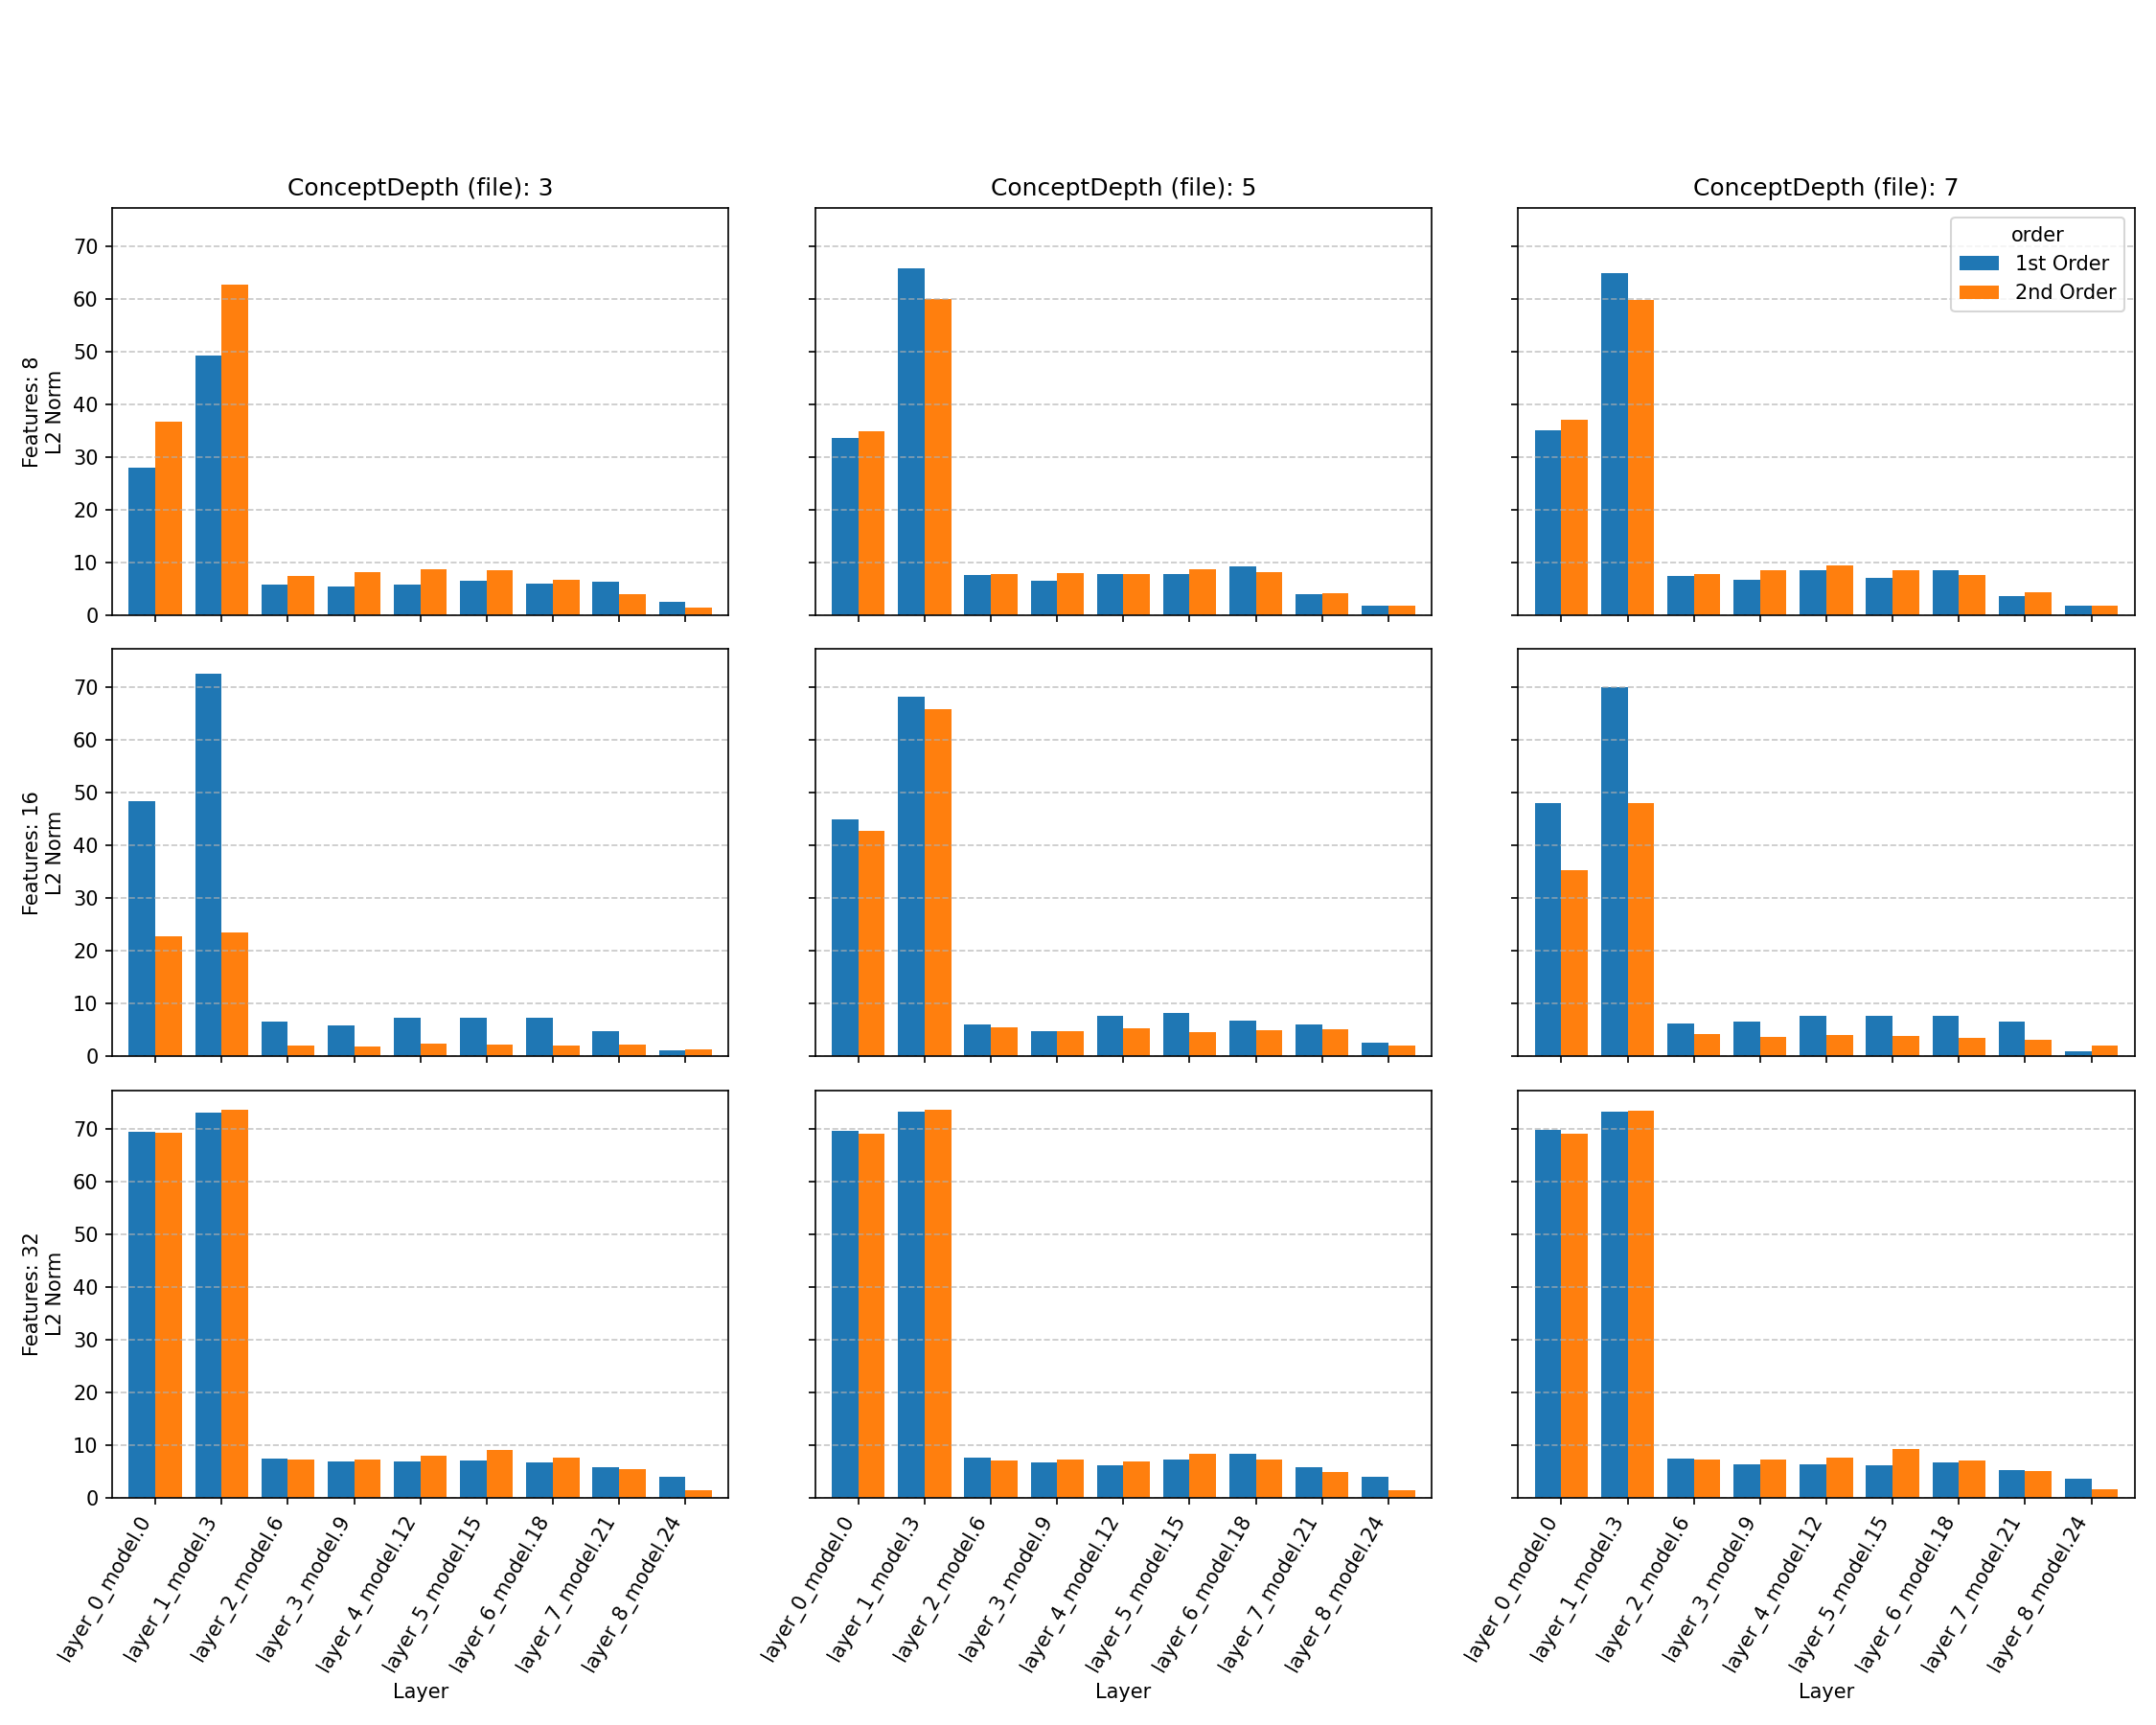
\includegraphics[width=0.8\textwidth]{Figures/faceted_norm_comparison_faceted_norm_comparison.png} 
    \caption{Average L2 Norm of MLP Layer Weights. Comparison of 1st-Order Meta-SGD and 2nd-Order Meta-SGD, faceted by input features (rows) and concept depth from filename (columns). Each bar group represents a layer within the MLP. Norms are averaged over available seeds for each configuration. The x-axis labels indicate the layer index. }
    \label{fig:layer_norms_faceted}
\end{figure}

\end{document}